\begin{figure}[h!]
    \centering
    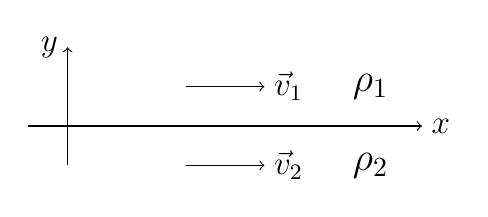
\begin{tikzpicture}
        \draw 
            [->, black] (-2,0)--(3,0) node[anchor=west]{\large $x$};
        \draw 
            [->, black] (-1.5, -0.5)--(-1.5, 1) node[anchor=east]{\large $y$};
        \draw 
            [->, black] (0,0.5)--(1,0.5) node[anchor=west]{\large $\vec{v}_{1}$};
        \draw 
            (2,0.5) node[anchor=west]{\Large $\rho_{1}$};
        \draw 
            [->, black] (0,-0.5)--(1,-0.5) node[anchor=west]{\large $\vec{v}_{2}$};
        \draw 
            (2,-0.5) node[anchor=west]{\Large $\rho_{2}$};
    \end{tikzpicture}
    \caption{Stratified fluids may give raise to instabilities.}
    \label{fig:stratified_fluid}
\end{figure}